\subsubsection{Variational Autoencoder (\acrshort{vae})}
\label{back:vae}

Similar to the regular autoencoder, a \acrfull{vae} also aims to map input over to a feature representation. The diffre. Broadly speaking, the difference between a AE and a \acrshort{vae} is that a AE maps input to points, where as VAEs map over to a distribution in the latent space. The encoder $E$ outputs to vectors. 

Thus, the \acrlong{vae} can be seemed as a generative model.


\begin{figure}[h]
    \centering
    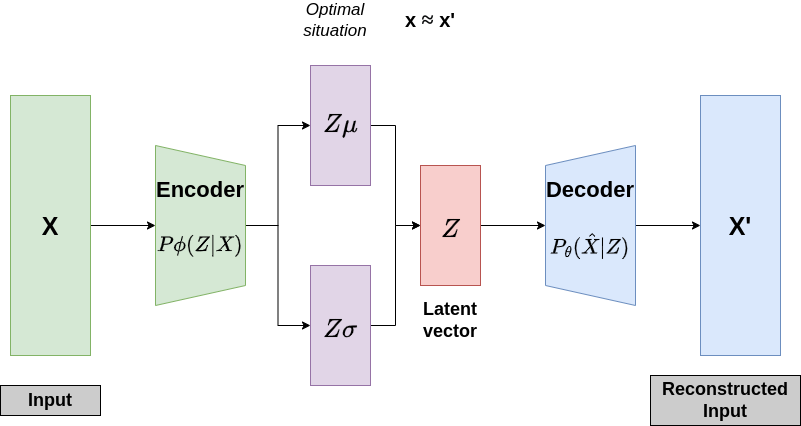
\includegraphics[scale=0.5]{figures/vae.png}
    \caption{Variational Autoencoder Architecture Diagram}
    \label{fig:vaediagram}
\end{figure}


VAEs can be trained by backpropagation due to something known as the \textit{reparametrization trick}. We need this because since VAEs maps to a stochastic variable, abckpropagation would else not be feasible.

\begin{align*}
\text{Given:} & \quad \text{Encoder LSTM outputs: } h \\
& \quad \text{Mean vector: } \mu \\
& \quad \text{Log variance vector: } \log(\sigma^2) \\
\text{Sample:} & \quad \epsilon \sim \mathcal{N}(0, 1) \\
\text{Reparameterization:} & \quad z = \mu + \sigma \odot \epsilon \\
\text{Decoder Input:} & \quad z \quad \text{(sampled latent vector)} \\
\text{Training Objective:} & \quad \text{Minimize reconstruction error} \\
& \quad \text{and KL divergence between } q(z|x) \text{ and } p(z) \\
\text{Loss Function:} & \quad \mathcal{L} = \text{reconstruction\_loss} + \text{KL\_divergence}
\end{align*}


\textbf{KEYS TO GETTING A GOOD VARIATIONAL AUTO ENCODER}

\begin{itemize}
    \item Pick the righ size for the latent space
    \item Learning rate scheduler  and hyperparam tuning 
    \item BETA COEFFICIENT
\end{itemize}

An effort has been made into trying to improve autoencoders for anomaly detection \cite{tan2023improving}

THIS ONE IS HIGHLY RELEVANT AND HAS MANY METRICS \cite{s23021009}